% Options for packages loaded elsewhere
\PassOptionsToPackage{unicode}{hyperref}
\PassOptionsToPackage{hyphens}{url}
%
\documentclass[
]{book}
\usepackage{lmodern}
\usepackage{amsmath}
\usepackage{ifxetex,ifluatex}
\ifnum 0\ifxetex 1\fi\ifluatex 1\fi=0 % if pdftex
  \usepackage[T1]{fontenc}
  \usepackage[utf8]{inputenc}
  \usepackage{textcomp} % provide euro and other symbols
  \usepackage{amssymb}
\else % if luatex or xetex
  \usepackage{unicode-math}
  \defaultfontfeatures{Scale=MatchLowercase}
  \defaultfontfeatures[\rmfamily]{Ligatures=TeX,Scale=1}
\fi
% Use upquote if available, for straight quotes in verbatim environments
\IfFileExists{upquote.sty}{\usepackage{upquote}}{}
\IfFileExists{microtype.sty}{% use microtype if available
  \usepackage[]{microtype}
  \UseMicrotypeSet[protrusion]{basicmath} % disable protrusion for tt fonts
}{}
\makeatletter
\@ifundefined{KOMAClassName}{% if non-KOMA class
  \IfFileExists{parskip.sty}{%
    \usepackage{parskip}
  }{% else
    \setlength{\parindent}{0pt}
    \setlength{\parskip}{6pt plus 2pt minus 1pt}}
}{% if KOMA class
  \KOMAoptions{parskip=half}}
\makeatother
\usepackage{xcolor}
\IfFileExists{xurl.sty}{\usepackage{xurl}}{} % add URL line breaks if available
\IfFileExists{bookmark.sty}{\usepackage{bookmark}}{\usepackage{hyperref}}
\hypersetup{
  pdftitle={Statistics with jamovi},
  pdfauthor={Dana Wanzer},
  hidelinks,
  pdfcreator={LaTeX via pandoc}}
\urlstyle{same} % disable monospaced font for URLs
\usepackage{longtable,booktabs}
% Correct order of tables after \paragraph or \subparagraph
\usepackage{etoolbox}
\makeatletter
\patchcmd\longtable{\par}{\if@noskipsec\mbox{}\fi\par}{}{}
\makeatother
% Allow footnotes in longtable head/foot
\IfFileExists{footnotehyper.sty}{\usepackage{footnotehyper}}{\usepackage{footnote}}
\makesavenoteenv{longtable}
\usepackage{graphicx}
\makeatletter
\def\maxwidth{\ifdim\Gin@nat@width>\linewidth\linewidth\else\Gin@nat@width\fi}
\def\maxheight{\ifdim\Gin@nat@height>\textheight\textheight\else\Gin@nat@height\fi}
\makeatother
% Scale images if necessary, so that they will not overflow the page
% margins by default, and it is still possible to overwrite the defaults
% using explicit options in \includegraphics[width, height, ...]{}
\setkeys{Gin}{width=\maxwidth,height=\maxheight,keepaspectratio}
% Set default figure placement to htbp
\makeatletter
\def\fps@figure{htbp}
\makeatother
\setlength{\emergencystretch}{3em} % prevent overfull lines
\providecommand{\tightlist}{%
  \setlength{\itemsep}{0pt}\setlength{\parskip}{0pt}}
\setcounter{secnumdepth}{5}
\usepackage{booktabs}

\newenvironment{danger}
    {
    \hline\\
    }
    { 
    \\\\\hline
    }
    
\newenvironment{warning}
    {
    \hline\\
    }
    { 
    \\\\\hline
    }
    
\newenvironment{info}
    {
    \hline\\
    }
    { 
    \\\\\hline
    }
    
\newenvironment{try}
    {
    \hline\\
    }
    { 
    \\\\\hline
    }
\ifluatex
  \usepackage{selnolig}  % disable illegal ligatures
\fi
\usepackage[]{natbib}
\bibliographystyle{apalike}

\title{Statistics with jamovi}
\author{Dana Wanzer}
\date{Last Update: 2020-10-31}

\begin{document}
\maketitle

{
\setcounter{tocdepth}{1}
\tableofcontents
}
\hypertarget{welcome}{%
\chapter*{Welcome}\label{welcome}}
\addcontentsline{toc}{chapter}{Welcome}

This is the website for PSYC 290 and PSYC 790 at the University of Wisconsin-Stout, taught by Dana Wanzer. These resources are aimed at teaching you how to use jamovi and null hypothesis significance testing (NHST) to answer research questions.

This website is \textbf{free to use} and is licensed under a Creative Commons BY-SA (CC BY-SA) license version 4.0. This means you are free to \textbf{share} (i.e., copy and redistribute the material in any medium or format) and \textbf{adapt} (i.e., remix, transform, and build upon the material for any purpose, even commercially), provided that you \textbf{attribute} these resources by citing me, indicating if changes were made and you \textbf{share alike} (i.e., if you adapt, you must distribute your contributes under the same license as the original).

Portions of this book may have been adapted from ``\href{http://www.learnstatswithjamovi.com}{Learning statistics with jamovi: A tutorial for psychology students and other beginners}'' by Danielle J. Navarro and David R. Foxcroft, version 0.70. Furthermore, the template and style of this book is from \href{https://psyteachr.github.io/book-template/setup.html}{PsyTeachR}.

\hypertarget{introduction}{%
\chapter{Introduction}\label{introduction}}

This chapter will walk you through how this website/book works.

\hypertarget{quiz-questions}{%
\section{Quiz Questions}\label{quiz-questions}}

Throughout this website, there will be questions to help you test your knowledge. When you type in or select the correct answer, the dashed box will change color and become solid.

For example:

\begin{itemize}
\item
  What is 2+2?
\item
  We attend the University of Wisconsin- Stout Madison Green Bay
\item
  True or false: Statistics is awesome. TRUE FALSE
\end{itemize}

\hypertarget{errors-and-mistakes}{%
\section{Errors and mistakes}\label{errors-and-mistakes}}

I am human, therefore I err. If you find an error in the textbook or something you think might be a mistake, please let me know ASAP so I can update this for everyone else. Let me know which section you find the error or mistake in and what the error or mistake is. For example, if there was an error here you could say, ``There was an error in 1.2 that the first sentence should really be `To err is human.'\,''

\hypertarget{independent-t-test}{%
\chapter{Independent t-test}\label{independent-t-test}}

\hypertarget{what-is-the-independent-t-test}{%
\section{What is the independent t-test?}\label{what-is-the-independent-t-test}}

The independent t-test is used to test the difference in our dependent variable between two different groups of observations. Our grouping variable is our independent variable. In other words, we use the independent t-test when we have a research question with a \textbf{continuous dependent variable} and a \textbf{categorical independent variable with two categories in which different participants are in each category}.

The independent t-test is also the independent samples t-test and the Student's t-test. I will use these terms interchangeably.

\hypertarget{data-set-up}{%
\section{Data set-up}\label{data-set-up}}

To conduct the independent t-test, we first need to ensure our data is set-up properly in our dataset. This requires having two columns: one with our continuous dependent variable and one indicating which group the participant is in. Each row is a unique participant or unit of analysis. Here's what example data may look like if we were testing for differences in a test score by students in my fall or spring semesters of this course:

\begin{longtable}[]{@{}llr@{}}
\caption{Example data for the independent t-test}\tabularnewline
\toprule
ID & Semester & TestScore\tabularnewline
\midrule
\endfirsthead
\toprule
ID & Semester & TestScore\tabularnewline
\midrule
\endhead
1 & Fall & 86\tabularnewline
2 & Fall & 80\tabularnewline
3 & Fall & 75\tabularnewline
4 & Fall & 79\tabularnewline
5 & Fall & 82\tabularnewline
6 & Spring & 84\tabularnewline
7 & Spring & 90\tabularnewline
8 & Spring & 72\tabularnewline
9 & Spring & 75\tabularnewline
10 & Spring & 81\tabularnewline
\bottomrule
\end{longtable}

In the example data above, what is your \textbf{independent variable}? ID Semester TestScore

In the example data above, what is your \textbf{dependent variable}? ID Semester TestScore

\hypertarget{the-math-behind-the-independent-t-test}{%
\section{The math behind the independent t-test}\label{the-math-behind-the-independent-t-test}}

The basic math of the independent t-test the mean difference divided by the pooled standard error.

\(t = \frac{\bar{X}_1 - \bar{X}_2}{SE({\bar{X}_1 - \bar{X}_2})}\)

The denominator of the equation is more difficult to calculate and depends on whether the sample size between groups is equal.

\hypertarget{assumptions}{%
\section{Assumptions}\label{assumptions}}

As a parametric test, the independent t-test has the same assumptions as other parametric tests:

\begin{enumerate}
\def\labelenumi{\arabic{enumi}.}
\item
  The dependent variable is \textbf{normally distributed}
\item
  Variances in the two groups are roughly equal (i.e., \textbf{homogeneity of variances})
\item
  The dependent variable is \textbf{interval or ratio} (i.e., continuous)
\item
  Scores are \textbf{independent} between groups
\end{enumerate}

We cannot \underline{test} the third and fourth assumptions; rather, those are based on knowing your data.

However, we can and should test for the first two assumptions. Fortunately, the independent samples t-test in jamovi has two check boxes under ``Assumption Checks'' that lets us test for both assumptions.

\hypertarget{in-jamovi}{%
\section{In jamovi}\label{in-jamovi}}

Let's run an example with data from lsj-data. Open data from your Data Library in ``lsj-data''. Select and open ``Harpo''. This dataset is hypothetical data of 33 students taking Dr.~Harpo's statistics lectures. We have two tutors for the class, Anastasia (\emph{n} = 15) and Bernadette (\emph{n} = 18). Our research question is ``Which tutor results in better student grades?'' We don't have a hypothesis that one does better than the other.

\begin{enumerate}
\def\labelenumi{\arabic{enumi}.}
\item
  To perform an independent t-test in jamovi, go to the Analyses tab, click the T-Tests button, and choose ``Independent Samples T-Test''.
\item
  Move your dependent variable \texttt{grade} to the Dependent Variables box and your independent variable \texttt{tutor} to the Grouping Variable box.
\item
  Under Tests, select \texttt{Student\textquotesingle{}s}
\item
  Under Hypothesis, because we have a two-sided hypothesis select a two-sided hypothesis (Group 1 does not equal Group 2).
\item
  Under Additional Statistics, select \texttt{Mean\ difference}, \texttt{Effect\ size}, and \texttt{Descriptives}.
\item
  Under Assumption Checks, select all three options: \texttt{Homogeneity\ test}, \texttt{Normality\ test}, and \texttt{Q-Q\ plot}.
\end{enumerate}

When you are done, your setup should look like this

\begin{figure}

{\centering 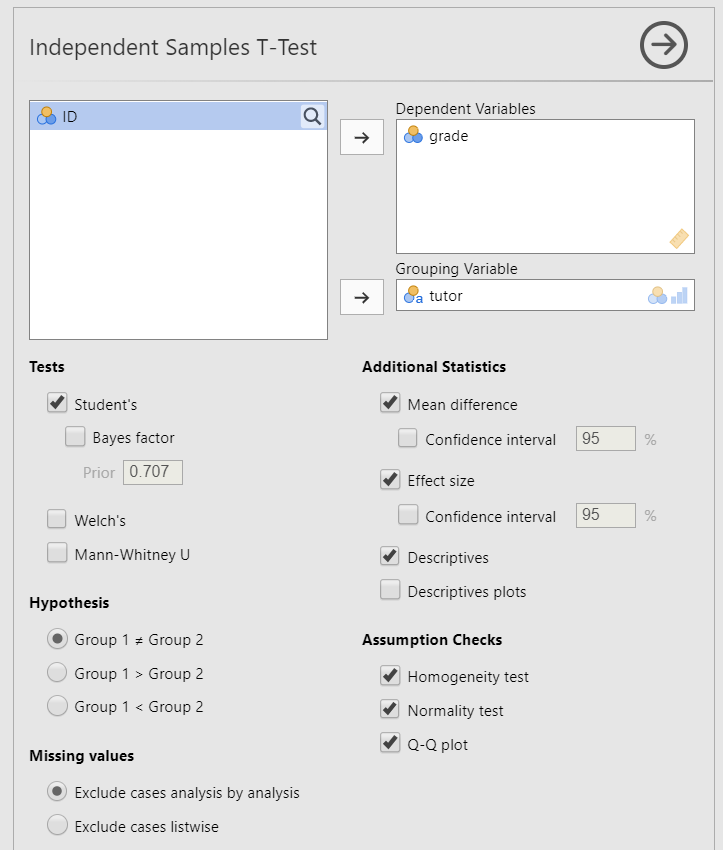
\includegraphics[width=0.8\linewidth]{images/02-independent_t-test/independent_t-test_setup} 

}

\caption{Independent t-test setup in jamovi}\label{fig:unnamed-chunk-1}
\end{figure}

\hypertarget{checking-assumptions-in-jamovi}{%
\subsection{Checking assumptions in jamovi}\label{checking-assumptions-in-jamovi}}

\hypertarget{testing-normality}{%
\subsubsection{Testing normality}\label{testing-normality}}

We test for normality using the Shapiro-Wilk test and the Q-Q plot. The Shapiro-Wilk test was not statistically significant (W = .98, \emph{p} = .827); therefore, this indicates the data is normally distributed. Furthermore, the lines are fairly close to the diagonal line in the Q-Q plot. We can conclude that we satisfy the assumption of normality.

\begin{figure}

{\centering 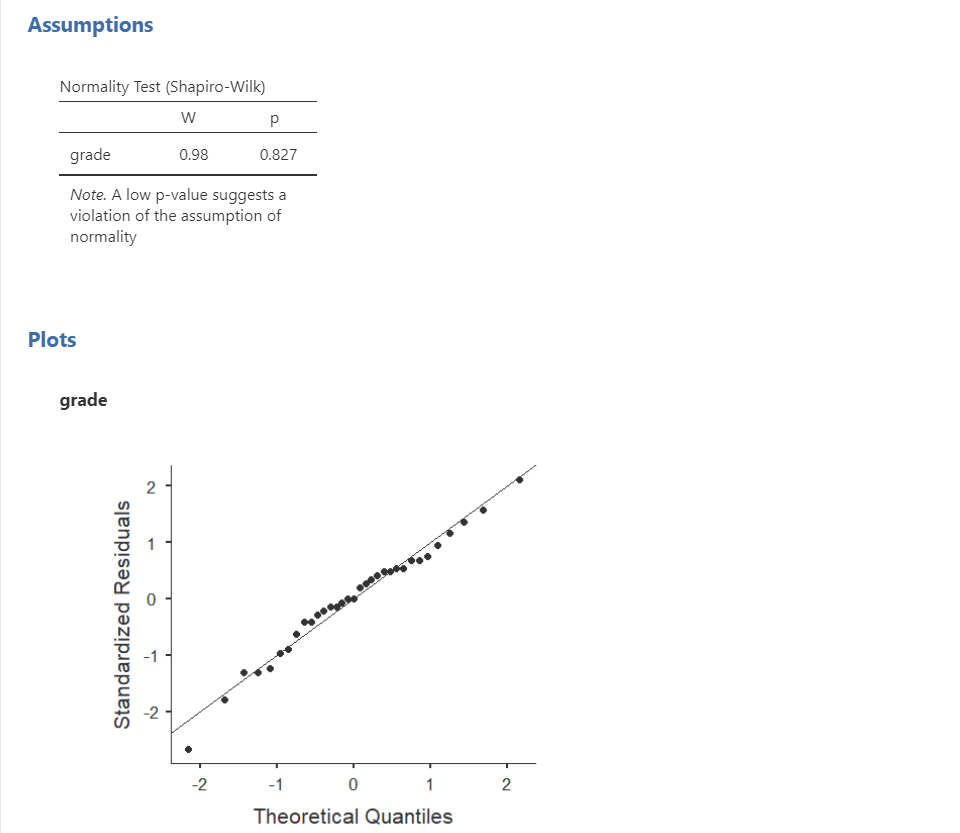
\includegraphics[width=1\linewidth]{images/02-independent_t-test/independent_t-test_normality} 

}

\caption{Testing normality in jamovi}\label{fig:unnamed-chunk-2}
\end{figure}

\hypertarget{testing-homogeneity-of-variance}{%
\subsubsection{Testing homogeneity of variance}\label{testing-homogeneity-of-variance}}

We test for homogeneity of variance using the Levene's test. The Levene's test was not statistically significant (\emph{F} {[}1, 31{]} = 2.49, \emph{p} = .125); therefore, this indicates our data satisfies the assumption of homogeneity of variance. However, I would add a caveat that we have a small sample of data (\emph{n} = 15 for Anastasia and \emph{n} = 18 for Bernadette) and the standard deviations are quite different from one another (SD = 9.00 vs 5.77, respectively). We should have tried to collect more data.

\begin{figure}

{\centering 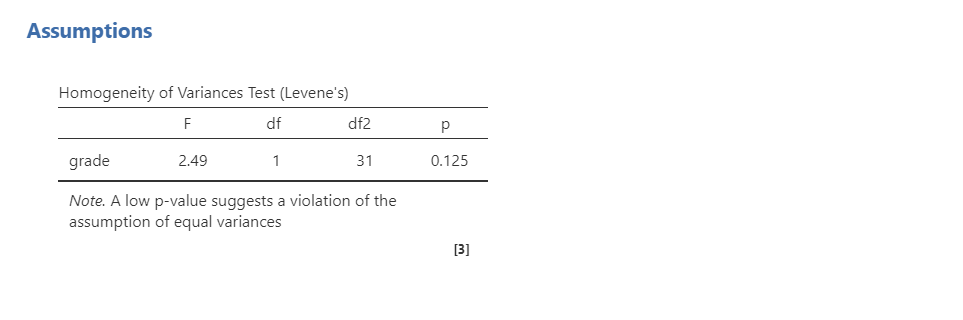
\includegraphics[width=1\linewidth]{images/02-independent_t-test/independent_t-test_homogeneity} 

}

\caption{Testing homogeneity of variance in jamovi}\label{fig:unnamed-chunk-3}
\end{figure}

\hypertarget{interpreting-results}{%
\subsection{Interpreting results}\label{interpreting-results}}

Once we are satisfied we have satisfied the assumptions for the independent t-test, we can interpret our results.

\begin{figure}

{\centering 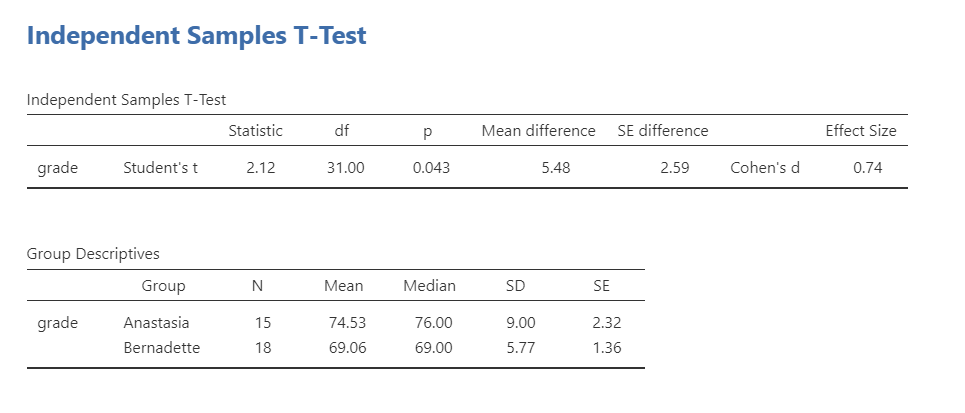
\includegraphics[width=1\linewidth]{images/02-independent_t-test/independent_t-test_ind-results} 

}

\caption{Independent t-test results in jamovi}\label{fig:unnamed-chunk-4}
\end{figure}

Our p-value is less than .05, so our results are statistically significant. We can write up our results in APA something like this:

\begin{quote}
Anastasia's students (\emph{M} = 74.53, \emph{SD} = 9.00, \emph{n} = 15) had significantly higher grades than Bernadette's students (\emph{M} = 69.06, \emph{SD} = 5.77, \emph{n}~= 18), \emph{t} (31) = 2.12, \emph{p} = .043, \emph{d} = .74.
\end{quote}

Sometimes, people like to put the statistics inside a parentheses. In that case, you need to change the parentheses around the degrees of freedom as brackets. Here's another example write-up of the results in APA style:

\begin{quote}
I tested the difference in grades between Anastasia's students (\emph{M} = 74.53, \emph{SD} = 9.00, \emph{n} = 15) and Bernadette's students (\emph{M} = 69.06, \emph{SD} = 5.77, \emph{n}~= 18). An independent samples t-test showed that the 5.48 mean difference between the tutor's student was statistically significant (\emph{t} {[}31{]} = 2.12, \emph{p} = .043, \emph{d} = .74).
\end{quote}

\hypertarget{additional-information-about-the-independent-t-test}{%
\section{Additional information about the independent t-test}\label{additional-information-about-the-independent-t-test}}

\hypertarget{positive-and-negative-t-values}{%
\subsection{Positive and negative t values}\label{positive-and-negative-t-values}}

Students often worry about positive or negative t-statistic values and are unsure how to interpret it. Positive or negative t-statistic values simply occur based on which group is listed first. Our t-statistic above is positive because we tested the difference between Anastasia and Bernadette: (Anastasia - Bernadette) = (74.53 - 69.06) = (5.48).

However, if we flipped it and tested the difference between Bernadette and Anastasia, our mean difference would be -5.48 and our t-statistic would be -2.12.

All that is to say, \emph{your positive or negative t-statistic is arbitrary}. So do not fret!

However, it is important the sign of your t-statistic matches what you report. For example, notice the difference:

\begin{quote}
\begin{enumerate}
\def\labelenumi{\arabic{enumi}.}
\tightlist
\item
  Anastasia's students had \textbf{higher} grades than Bernadette's, \emph{t} (31) = \textbf{2.12}, \emph{p} = .043, \emph{d} = .74.
\item
  Bernadette's students had \textbf{lower} grades than Anastasia's, \emph{t} (31) = \textbf{-2.12}, \emph{p} = .043, \emph{d} = .74.
\end{enumerate}
\end{quote}

One last note: this positive or negative t-statistic is only relevant for the independent and dependent t-test. You will not get negative values for the F-statistic or chi-square tests!

\hypertarget{what-if-i-violated-assumptions}{%
\subsection{What if I violated assumptions?}\label{what-if-i-violated-assumptions}}

The great news is that jamovi includes the Welch's t-statistic and the non-parametric version of the independent t-test (Mann-Whitney U)! The Welch's t-test has three main differences from the independent samples t-test: (a) the standard error (SE) is not a pooled estimate, (b) the degrees of freedom are calculated very different (not \emph{N} - 2), and (c) it does not have an assumption of homogeneity of variance. The Mann-Whitney U is not calculated based on the mean but rather the median and compares ranks of values across the two groups: it has no assumptions about the distribution of data or homogeneity of variances.

Here's what statistic you should choose based on satisfying assumptions:

\begin{longtable}[]{@{}lll@{}}
\toprule
\begin{minipage}[b]{0.39\columnwidth}\raggedright
\strut
\end{minipage} & \begin{minipage}[b]{0.25\columnwidth}\raggedright
\textbf{Normality: satisfied}\strut
\end{minipage} & \begin{minipage}[b]{0.27\columnwidth}\raggedright
\textbf{Normality: not satisfied}\strut
\end{minipage}\tabularnewline
\midrule
\endhead
\begin{minipage}[t]{0.39\columnwidth}\raggedright
\textbf{Homogeneity of Variance: satisfied}\strut
\end{minipage} & \begin{minipage}[t]{0.25\columnwidth}\raggedright
independent samples t-test\strut
\end{minipage} & \begin{minipage}[t]{0.27\columnwidth}\raggedright
Mann-Whitney U\strut
\end{minipage}\tabularnewline
\begin{minipage}[t]{0.39\columnwidth}\raggedright
\textbf{Homogeneity of Variance: not satisfied}\strut
\end{minipage} & \begin{minipage}[t]{0.25\columnwidth}\raggedright
Welch's t-test\strut
\end{minipage} & \begin{minipage}[t]{0.27\columnwidth}\raggedright
Mann-Whitney U\strut
\end{minipage}\tabularnewline
\bottomrule
\end{longtable}

Here is what the output for all three tests look like:

\begin{figure}

{\centering 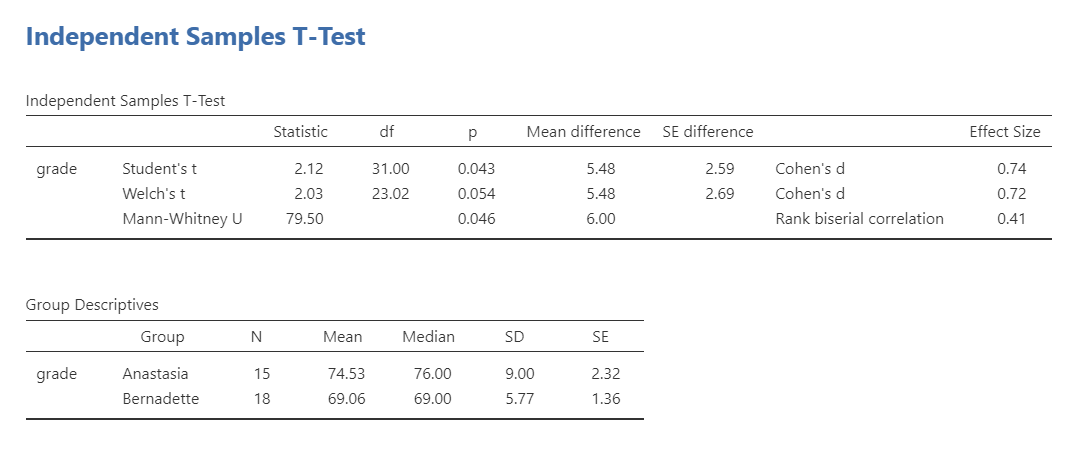
\includegraphics[width=1\linewidth]{images/02-independent_t-test/independent_t-test_full-results} 

}

\caption{All independent t-test results in jamovi}\label{fig:unnamed-chunk-5}
\end{figure}

\hypertarget{welchs-t-test-in-jamovi}{%
\subsubsection{Welch's t-test in jamovi}\label{welchs-t-test-in-jamovi}}

To conduct this in jamovi, under Tests select \texttt{Welch\textquotesingle{}s}. You will interpret the results similarly to the independent t-test:

\begin{quote}
Using a Welch's t-test, there was not a statistically significant difference in grades between Anastasia's students (\emph{M} = 74.53, \emph{SD} = 9.00, \emph{n} = 15) and Bernadette's students (\emph{M} = 69.06, \emph{SD} = 5.77, \emph{n} = 18), \emph{t} (23.02) = 2.03, \emph{p} = .054, \emph{d} = .72.
\end{quote}

Why is it no longer statistically significant? Which result should you trust? In reality, the difference in \emph{p}-values is likely due to chance. However, the independent t-test and Welch's test have different strengths and weaknesses. If the two populations really do have equal variances, then the independent t-test is slightly more powerful (lower Type II error rate) than the Welch's test. However, if they \emph{don't} have the same variances, then the assumptions of the independent t-test are violated and you may not be able to trust the results; you may end up with a higher Type I error rate. So it's a trade-off.

Which should you use? I tend to prefer always using Welch's t-test because if the variances are equal, then there will be practically no difference between the independent and Welch's t-test. But if the variances are not equal, then Welch's t-test will outperform the independent t-test. For that reason, defaulting to the Welch's t-test makes most sense to me.

\hypertarget{mann-whitney-u-test}{%
\subsubsection{Mann-Whitney U test}\label{mann-whitney-u-test}}

If you do not satisfy the assumption of normality (regardless of whether you satisfy the assumption of homogeneity of variance), you should either try to transform your data to be normally distributed or you will need to use a non-parametric test. In this case, if you originally wanted to perform an independent t-test, the non-parametric equivalent test is the Mann-Whitney U test.

I will not go into specifics, but the idea behind the Mann-Whitney U test is that you take all the values (regardless of group) and rank them. You then sum the ranks across groups and calculate your U statistic and p-value. You interpret the p-value like you normally would, but there are differences in how we report the results because this statistic is based on the \emph{median} not the \emph{mean}.

\begin{quote}
Using the Mann-Whitney U test, there was a statistically significant difference in grades between Anastasia's students (\emph{Mdn} = 76, \emph{n} = 15) and Bernadette's students (\emph{Mdn} = 69, \emph{n}~= 18), \emph{t} (23.02) = 2.03, \emph{p} = .054, \emph{d} = .72.
\end{quote}

\hypertarget{your-turn}{%
\section{Your turn!}\label{your-turn}}

Open the \texttt{Sample\_Dataset\_2014.xlsx} file that we will be using for all Your Turn exercises.

Perform independent t-tests based on the following research questions. Think critically about whether you should be using a one-tailed or two-tailed hypothesis and check your assumptions so you know which test to use!

To get the most out of these exercises, try to first find out the answer on your own and then use the drop-down menus to check your answer.

\begin{enumerate}
\def\labelenumi{\arabic{enumi}.}
\item
  \textbf{Does height differ by gender (Gender: male = 0, female = 1)?}

  \begin{itemize}
  \item
    Should you use a one-tailed or two-tailed hypothesis? one-tailed two-tailed
  \item
    Which statistic should you use based on your assumptions? independent t-test Welch's t-test Mann Whitney U
  \item
    Does height differ by gender? yes no
  \end{itemize}
\item
  \textbf{Do athletes (Athlete: athletes = 1, non-athlete = 0) have faster sprint times than non-athletes?}

  \begin{itemize}
  \item
    Should you use a one-tailed or two-tailed hypothesis? one-tailed two-tailed
  \item
    Which statistic should you use based on your assumptions? independent t-test Welch's t-test Mann Whitney U
  \item
    Do athletes have faster sprint times than non-athletes? yes no
  \end{itemize}
\item
  \textbf{Do students who live on campus (LiveOnCampus: on campus = 1, off campus = 0) have higher English scores than students who live off campus?}

  \begin{itemize}
  \item
    Should you use a one-tailed or two-tailed hypothesis? one-tailed two-tailed
  \item
    Which statistic should you use based on your assumptions? independent t-test Welch's t-test Mann Whitney U
  \item
    Does students who live on campus have higher English scores? yes no
  \end{itemize}
\item
  \textbf{Does athletic status relate to math scores?}

  \begin{itemize}
  \item
    Should you use a one-tailed or two-tailed hypothesis? one-tailed two-tailed
  \item
    Which statistic should you use based on your assumptions? independent t-test Welch's t-test Mann Whitney U
  \item
    Does athletic status relate to math scores? yes no
  \end{itemize}
\end{enumerate}

\hypertarget{dependent-t-test}{%
\chapter{Dependent t-test}\label{dependent-t-test}}

\hypertarget{what-is-the-dependent-t-test}{%
\section{What is the dependent t-test?}\label{what-is-the-dependent-t-test}}

The dependent t-test is used to test the difference in our dependent variable between two categories in which participants are the \emph{same} across categories. Our category variable is our independent variable. In other words, we use the independent t-test when we have a research question with a \textbf{continuous dependent variable} and a \textbf{categorical independent variable with two categories in which the same participants are in each category}.

The dependent t-test is also called a dependent samples t-test or paired samples t-test.

\hypertarget{data-set-up-1}{%
\section{Data set-up}\label{data-set-up-1}}

To conduct the dependent t-test, we first need to ensure our data is set-up properly in our dataset. This requires having two columns: one is our dependent variable score for the participant in one category and the other column is our dependent variable score for the participant in the other category. Each row is a unique participant or unit of analysis. Here's what example data may look like if we were testing for differences in test scores across the same participants in the fall and spring:

\begin{longtable}[]{@{}llr@{}}
\caption{Example data for the dependent t-test}\tabularnewline
\toprule
ID & TestScore\_Fall & TestScore\_Spring\tabularnewline
\midrule
\endfirsthead
\toprule
ID & TestScore\_Fall & TestScore\_Spring\tabularnewline
\midrule
\endhead
1 & 75 & 86\tabularnewline
2 & 79 & 80\tabularnewline
3 & 65 & 75\tabularnewline
4 & 81 & 79\tabularnewline
5 & 73 & 82\tabularnewline
6 & 72 & 84\tabularnewline
7 & 69 & 90\tabularnewline
8 & 60 & 72\tabularnewline
9 & 75 & 75\tabularnewline
10 & 74 & 81\tabularnewline
\bottomrule
\end{longtable}

In the example data above, what is your \textbf{independent variable}? ID Semester TestScore

In the example data above, what is your \textbf{dependent variable}? ID Semester Test Score

\hypertarget{the-math-behind-the-independent-t-test-1}{%
\section{The math behind the independent t-test}\label{the-math-behind-the-independent-t-test-1}}

The basic math of the dependent t-test is the mean difference divided by the standard error, which is estimated based on the standard deviation and sample size (N).

\(t = \frac{\bar{X}_1 - \bar{X}_2}{s_d/ \sqrt{N}}\)

\hypertarget{assumptions-1}{%
\section{Assumptions}\label{assumptions-1}}

As a parametric test, the independent t-test has the same assumptions as other parametric tests minus the homogeneity of variance assumption because we are dealing with the same people across categories

\begin{enumerate}
\def\labelenumi{\arabic{enumi}.}
\item
  The \emph{differences in scores} in the dependent variable are \textbf{normally distributed}
\item
  The dependent variable is \textbf{interval or ratio} (i.e., continuous)
\item
  Scores are \textbf{independent} across participants
\end{enumerate}

We cannot \underline{test} the second and third assumptions; rather, those are based on knowing your data.

However, we can and should test for the first assumption. Fortunately, the dependent samples t-test in jamovi has two check boxes under ``Assumption Checks'' that lets us test normality.

\hypertarget{in-jamovi-1}{%
\section{In jamovi}\label{in-jamovi-1}}

Let's run an example with data from lsj-data. Open data from your Data Library in ``lsj-data''. Select and open ``Chico''. This dataset is hypothetical data from Dr.~Chico's class in which students took two tests: one early in the semester and one later in the semester. Dr.~Chico thinks that the first test is a ``wake up call'' for students. When they realise how hard her class really is, they'll work harder for the second test and get a better mark. Is she right? Let's test it!

\begin{enumerate}
\def\labelenumi{\arabic{enumi}.}
\item
  To perform an dependent t-test in jamovi, go to the Analyses tab, click the T-Tests button, and choose ``Paired Samples T-Test''.
\item
  Move both measurements of your dependent variable (\texttt{grade\_test1} and \texttt{grade\_test2}) to the Paired Variables box.
\item
  Under Tests, select \texttt{Student\textquotesingle{}s}
\item
  Under Hypothesis, choose the correct hypothesis: Measure 1 is not equal to Measure 2 Measure 1 \textgreater{} Measure 2 Measure 1 \textless{} Measure 2
\item
  Under Additional Statistics, select \texttt{Mean\ difference}, \texttt{Effect\ size}, and \texttt{Descriptives}.
\item
  Under Assumption Checks, select both options: \texttt{Normality\ test} and \texttt{Q-Q\ plot}.
\end{enumerate}

When you are done, your setup should look like this

\begin{figure}

{\centering 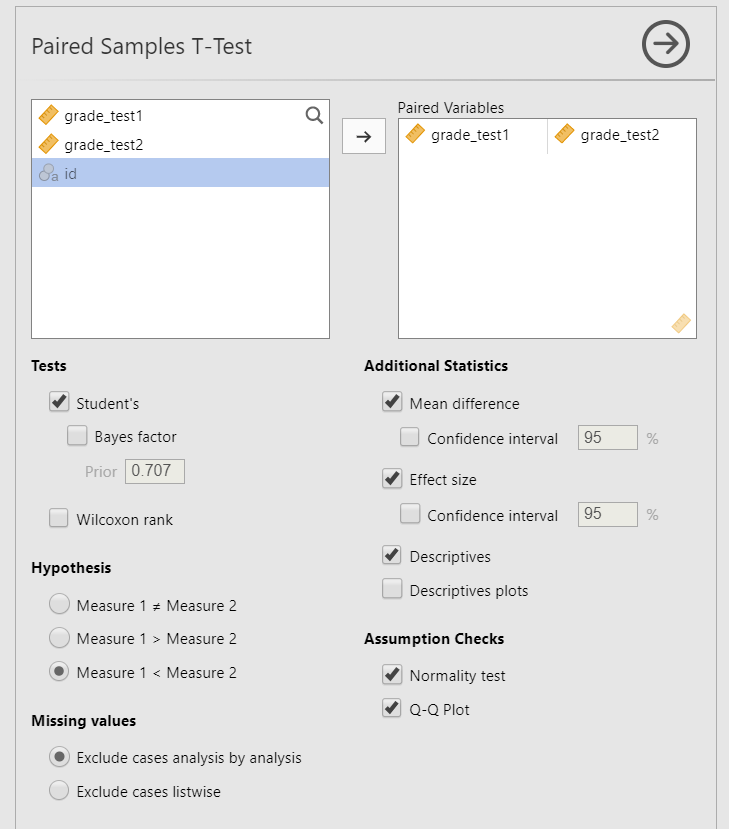
\includegraphics[width=0.8\linewidth]{images/03_dependent_t-test/dependent_setup} 

}

\caption{Dependent t-test setup in jamovi}\label{fig:unnamed-chunk-1}
\end{figure}

\hypertarget{checking-assumptions-in-jamovi-1}{%
\subsection{Checking assumptions in jamovi}\label{checking-assumptions-in-jamovi-1}}

\hypertarget{testing-normality-1}{%
\subsubsection{Testing normality}\label{testing-normality-1}}

We test for normality using the Shapiro-Wilk test and the Q-Q plot. The Shapiro-Wilk test was not statistically significant (W = .97, \emph{p} = .678); therefore, this indicates the data is normally distributed. Furthermore, the lines are fairly close to the diagonal line in the Q-Q plot (although it's a bit hard to tell because our sample size is small). We can conclude that we satisfy the assumption of normality.

\begin{figure}

{\centering 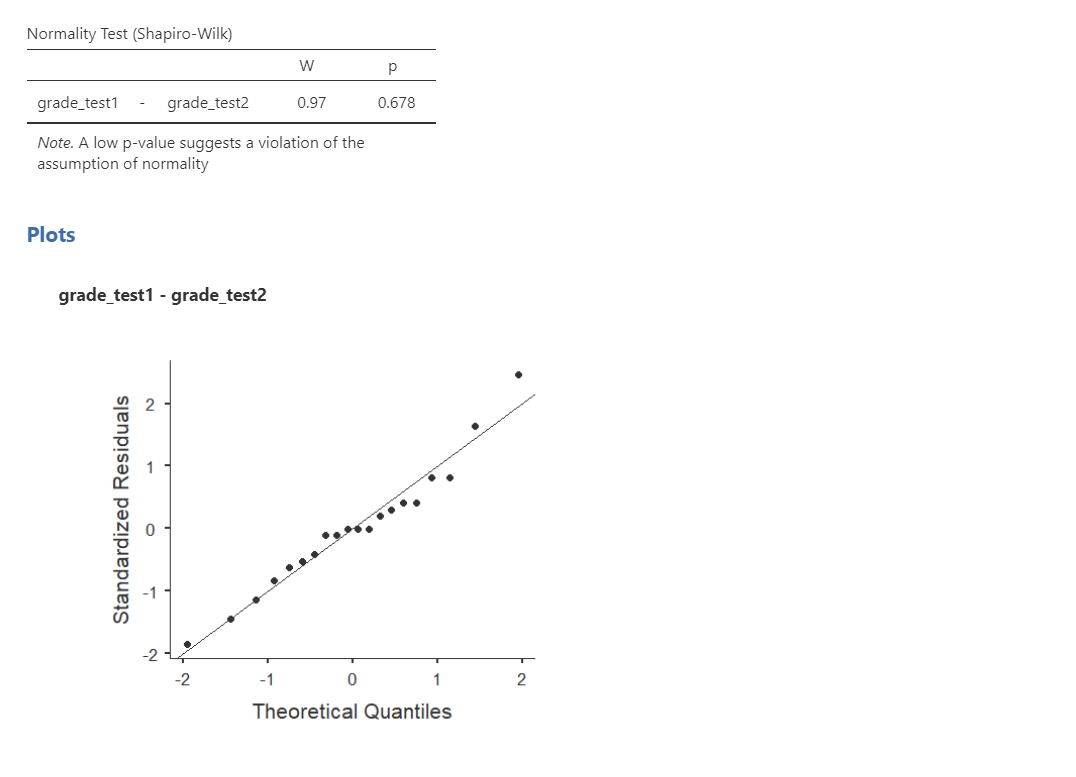
\includegraphics[width=1\linewidth]{images/03_dependent_t-test/dependent_normality} 

}

\caption{Testing normality in jamovi}\label{fig:unnamed-chunk-2}
\end{figure}

\hypertarget{interpreting-results-1}{%
\subsection{Interpreting results}\label{interpreting-results-1}}

Once we are satisfied we have satisfied the assumptions for the dependent t-test, we can interpret our results.

\begin{figure}

{\centering 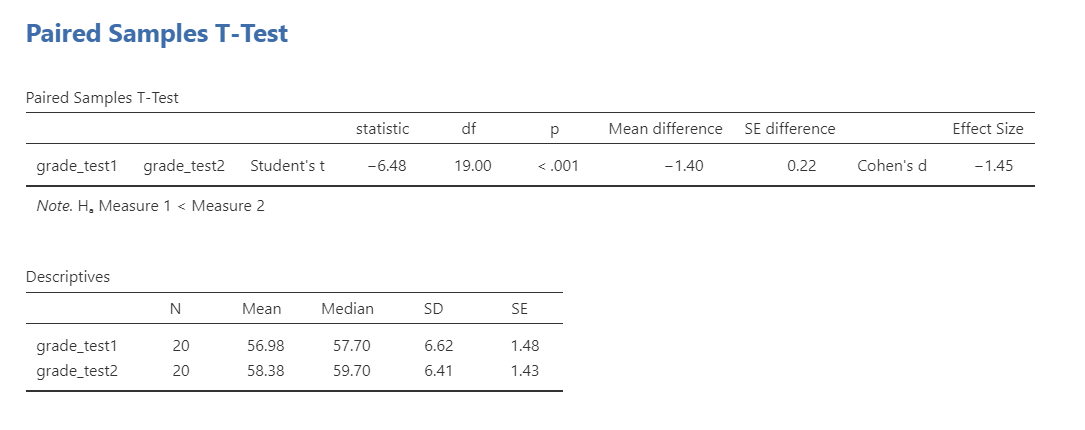
\includegraphics[width=1\linewidth]{images/03_dependent_t-test/dependent_results} 

}

\caption{Dependent t-test results in jamovi}\label{fig:unnamed-chunk-3}
\end{figure}

Our p-value is less than .05, so our results are statistically significant. We can write up our results in APA something like this:

\begin{quote}
The 20 students in Dr.~Chico's class performed worse on the first test (\emph{M} = 56.98, \emph{SD} = 6.62) than they did on the second test (\emph{M} = 58.38, \emph{SD} = 6.41), \emph{t}(19) = -6.48, \emph{p} \textless{} .001, \emph{d} = -1.45.
\end{quote}

Remember in the previous chapter that our t-test can be negative but we can always flip the interpretation. Here's another example of how we could write-up our results in APA style:

\begin{quote}
Dr.~Chico's hypothesis was correct in that her 20 students performed better on the second test (\emph{M} = 58.38, \emph{SD} = 6.41) than they did on the first test (\emph{M} = 56.98, \emph{SD} = 6.62), \emph{t}(19) = 6.48, \emph{p} \textless{} .001, \emph{d} = 1.45.
\end{quote}

\hypertarget{what-if-i-violated-assumptions-1}{%
\section{What if I violated assumptions?}\label{what-if-i-violated-assumptions-1}}

If you violated the assumption of normality and no transformation fixed your data, then you can perform the non-parametric version of the dependent t-test called the Wilcoxon Rank test. As a reminder, non-parametric tests do not make assumptions about the distribution of data because it deals with the \emph{median} not the \emph{mean}.

Here is the output for both the dependent t-test and the Wilcoxon rank test:

\begin{figure}

{\centering 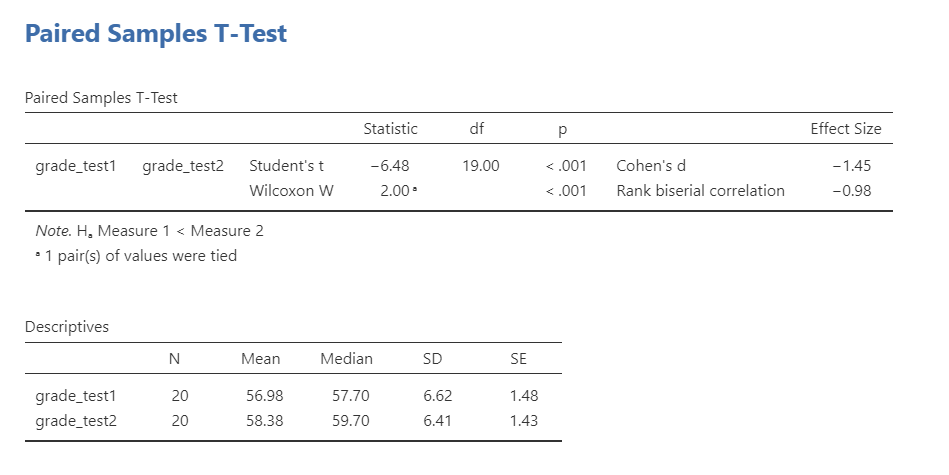
\includegraphics[width=1\linewidth]{images/03_dependent_t-test/dependent_results_full} 

}

\caption{All independent t-test results in jamovi}\label{fig:unnamed-chunk-4}
\end{figure}

\hypertarget{wilcoxon-rank-in-jamovi}{%
\subsubsection{Wilcoxon rank in jamovi}\label{wilcoxon-rank-in-jamovi}}

To conduct this in jamovi, under Tests select \texttt{Wilcoxon\ rank}. You will interpret the results similarly to the dependent t-test:

\begin{quote}
Using Wilcoxon rank test, students' test scores were significantly higher at the second test (\emph{Mdn} = 59.70) than at the first test (\emph{Mdn} = 57.70), W = 2.00, \emph{p} \textless{} .001.
\end{quote}

The note about tied values is not necessary to discuss. It is just telling us one participant had identical values for both test1 and test2 (student15).

\hypertarget{your-turn-1}{%
\section{Your turn!}\label{your-turn-1}}

Open the \texttt{Sample\_Dataset\_2014.xlsx} file that we use for all Your Turn exercises.

Perform dependent t-tests based on the following research questions. Think critically about whether you should be using a one-tailed or two-tailed hypothesis and check your assumptions so you know which test to use!

To get the most out of these exercises, try to first find out the answer on your own and then use the drop-down menus to check your answer.

\textbf{Note}: Technically, none of our data is suitable for a dependent t-test in this dataset. We will pretend that the four test score variables (\texttt{English}, \texttt{Reading}, \texttt{Math}, and \texttt{Writing}) are really four measurements of the same underlying test. In reality, we would analyze this data using correlation.

\begin{enumerate}
\def\labelenumi{\arabic{enumi}.}
\item
  \textbf{Do students perform better on the English test than they do the Writing test?}

  \begin{itemize}
  \item
    Should you use a one-tailed or two-tailed hypothesis? one-tailed two-tailed
  \item
    Which statistic should you use based on your assumptions? dependent t-test Wilcoxon rank
  \item
    Do students perform better on the English test than they do the Writing test? yes no
  \end{itemize}
\item
  \textbf{Does students' English scores relate to their Reading scores?}

  \begin{itemize}
  \item
    Should you use a one-tailed or two-tailed hypothesis? one-tailed two-tailed
  \item
    Which statistic should you use based on your assumptions? dependent t-test Wilcoxon rank
  \item
    Does students' English scores relate to their Reading scores? yes no
  \end{itemize}
\end{enumerate}

\hypertarget{one-way-anova}{%
\chapter{One-way ANOVA}\label{one-way-anova}}

\hypertarget{what-is-the-one-way-anova}{%
\section{What is the one-way ANOVA?}\label{what-is-the-one-way-anova}}

The one-way analysis of variance (ANOVA) is used to test the difference in our dependent variable between \underline{three or more} different groups of observations. Our grouping variable is our independent variable. In other words, we use the one-way ANOVA when we have a research question with a \textbf{continuous dependent variable} and a \textbf{categorical independent variable with three or more categories in which different participants are in each category}.

The one-way ANOVA is also known as an independent factor ANOVA.

One thing to keep in mind is the one-way ANOVA is an omnibus statistic that tests against the null hypothesis that the three or more means are the same. It does not tell us where the mean differences are (e.g., that 1 \textgreater{} 2); for that, we need planned contrasts or post-hoc procedures, which you'll learn about later.

\hypertarget{data-set-up-2}{%
\section{Data set-up}\label{data-set-up-2}}

To conduct the independent t-test, we first need to ensure our data is set-up properly in our dataset. This requires having two columns: one with our continuous dependent variable and one indicating which group the participant is in. Each row is a unique participant or unit of analysis. Here's what example data may look like if we were testing for differences in a test score by students in my fall, spring, or summer semesters of my course

\begin{longtable}[]{@{}llr@{}}
\caption{Example data for the one-way ANOVA}\tabularnewline
\toprule
\begin{minipage}[b]{0.29\columnwidth}\raggedright
ID\strut
\end{minipage} & \begin{minipage}[b]{0.29\columnwidth}\raggedright
Semester\strut
\end{minipage} & \begin{minipage}[b]{0.30\columnwidth}\raggedleft
TestScore\strut
\end{minipage}\tabularnewline
\midrule
\endfirsthead
\toprule
\begin{minipage}[b]{0.29\columnwidth}\raggedright
ID\strut
\end{minipage} & \begin{minipage}[b]{0.29\columnwidth}\raggedright
Semester\strut
\end{minipage} & \begin{minipage}[b]{0.30\columnwidth}\raggedleft
TestScore\strut
\end{minipage}\tabularnewline
\midrule
\endhead
\begin{minipage}[t]{0.29\columnwidth}\raggedright
1\strut
\end{minipage} & \begin{minipage}[t]{0.29\columnwidth}\raggedright
Fall\strut
\end{minipage} & \begin{minipage}[t]{0.30\columnwidth}\raggedleft
86\strut
\end{minipage}\tabularnewline
\begin{minipage}[t]{0.29\columnwidth}\raggedright
2\strut
\end{minipage} & \begin{minipage}[t]{0.29\columnwidth}\raggedright
Fall\strut
\end{minipage} & \begin{minipage}[t]{0.30\columnwidth}\raggedleft
80\strut
\end{minipage}\tabularnewline
\begin{minipage}[t]{0.29\columnwidth}\raggedright
3\strut
\end{minipage} & \begin{minipage}[t]{0.29\columnwidth}\raggedright
Fall\strut
\end{minipage} & \begin{minipage}[t]{0.30\columnwidth}\raggedleft
75\strut
\end{minipage}\tabularnewline
\begin{minipage}[t]{0.29\columnwidth}\raggedright
4\strut
\end{minipage} & \begin{minipage}[t]{0.29\columnwidth}\raggedright
Spring\strut
\end{minipage} & \begin{minipage}[t]{0.30\columnwidth}\raggedleft
79\strut
\end{minipage}\tabularnewline
\begin{minipage}[t]{0.29\columnwidth}\raggedright
5\strut
\end{minipage} & \begin{minipage}[t]{0.29\columnwidth}\raggedright
Spring\strut
\end{minipage} & \begin{minipage}[t]{0.30\columnwidth}\raggedleft
82\strut
\end{minipage}\tabularnewline
\begin{minipage}[t]{0.29\columnwidth}\raggedright
6\strut
\end{minipage} & \begin{minipage}[t]{0.29\columnwidth}\raggedright
Spring\strut
\end{minipage} & \begin{minipage}[t]{0.30\columnwidth}\raggedleft
84\strut
\end{minipage}\tabularnewline
\begin{minipage}[t]{0.29\columnwidth}\raggedright
7\strut
\end{minipage} & \begin{minipage}[t]{0.29\columnwidth}\raggedright
Summer\strut
\end{minipage} & \begin{minipage}[t]{0.30\columnwidth}\raggedleft
90\strut
\end{minipage}\tabularnewline
\begin{minipage}[t]{0.29\columnwidth}\raggedright
8\strut
\end{minipage} & \begin{minipage}[t]{0.29\columnwidth}\raggedright
Summer\strut
\end{minipage} & \begin{minipage}[t]{0.30\columnwidth}\raggedleft
72\strut
\end{minipage}\tabularnewline
\begin{minipage}[t]{0.29\columnwidth}\raggedright
9\strut
\end{minipage} & \begin{minipage}[t]{0.29\columnwidth}\raggedright
Summer\strut
\end{minipage} & \begin{minipage}[t]{0.30\columnwidth}\raggedleft
75\strut
\end{minipage}\tabularnewline
\bottomrule
\end{longtable}

In the example data above, what is your \textbf{independent variable}? ID Semester TestScore

In the example data above, what is your \textbf{dependent variable}? ID Semester TestScore

\hypertarget{why-not-multiple-t-tests}{%
\section{Why not multiple t-tests?}\label{why-not-multiple-t-tests}}

In the example above, we have three groups: fall, spring, and summer. We could just perform three separate t-tests: fall vs.~spring, fall vs.~summer, and spring vs.~summer.

However, the reason we do not perform multiple t-tests is to reduce our Type I error rate. If I had performed three separate t-tests, set my alpha (Type I error rate) at 5\%, and knew for a fact the effects do not actually exist, then each test has a probability of a Type I error rate of 5\%. Because we are running three tests, our alpha rate actually becomes 1 - (.95\textsuperscript{3})= 1 - .857 = 14.3\%! So now our \emph{familywise} or \emph{experimentwise}~error rate is 14.3\%, not the 5\% we originally set alpha at.

With three groups, that's not so bad, but let's see what happens with more tests we perform:

\begin{itemize}
\tightlist
\item
  \textbf{1 test}: 1 - (.95\textsuperscript{1})= 1 - .95 = \textbf{5\%}
\item
  \textbf{2 tests}: 1 - (.95\textsuperscript{2})= 1 - .9025 = \textbf{9.8\%}
\item
  \textbf{3 tests}: 1 - (.95\textsuperscript{3})= 1 - .857 = \textbf{14.3\%}
\item
  \textbf{4 tests}: 1 - (.95\textsuperscript{4})= 1 - .814 = \textbf{18.6\%}
\item
  \textbf{5 tests}: 1 - (.95\textsuperscript{5})= 1 - .774 = \textbf{22.6\%}
\item
  \textbf{10 tests}: 1 - (.95\textsuperscript{10})= 1 - .598 = \textbf{40.1\%}
\item
  \textbf{20 tests}: 1 - (.95\textsuperscript{20})= 1 - .358 = \textbf{64.1\%}
\end{itemize}

Ouch! 10 tests would have a Type I error rate of 40\%! That means that if we performed 10 statistical tests (assuming the effect does not exist), then 40\% of the results would be statistically significant by chance alone and would be a false positive. That's not good!

Therefore, we use the one-way ANOVA as one test to see if there is a difference overall. We can also do things to control or limit our familywise error rate, which I'll get into later.

\hypertarget{the-math-behind-the-one-way-anova}{%
\section{The math behind the one-way ANOVA}\label{the-math-behind-the-one-way-anova}}

The basic math of the one-way ANOVA is the between-group variance (mean squares - between groups) divided by the within-group variance (mean squares - within groups).

\(F = \frac{BG \:variance}{WG \:variance} = \frac{MS_{BG}}{MS_{WG}} = \frac{\frac{SS_{BG}}{df_{BG}}}{\frac{SS_{WG}}{df_{WG}}}\)

There are specific formulas for the between-group (also called the model) sum of squares (SS) and within-group (also called the residual) sum of squares. Keep in mind the following symbols:

\begin{itemize}
\tightlist
\item
  n/N = sample size (little n is per group, big N is the overall sample)
\item
  k = number of groups
\item
  X = mean
\item
  s = standard deviation
\end{itemize}

The between-group SS is the \emph{variation between group means}. The calculations you see below is to subtract the overall mean (\(\bar{X}_{grand}\)) from the group mean (\(\bar{X_k}\)), square that mean difference, multiply that by the sample size in that group (\(n_k\)), and then sum all the results of doing that per group.

\(SS_{BG} = \sum{n_k}(\bar{X_k}-\bar{X}_{grand})^2\)

\(df_{BG} = k - 1\)

The within-group SS is the \emph{variation of scores within groups}. The calculations you see below is to take the sample size in that group (\(n_k\)) and subtract 1 from it, then multiply it by the group's variance (\(s_k^2\), which is standard deviation squared), and then sum all the results of doing that per group.

\(SS_{WG} = \sum{s_k^2}(n_k - 1)\)

\(df_{WG} = N - k\)

In other words, the F-ratio is a ratio of the group or experimental effect by the individual differences in performance.

For our F-ratio to be statistically significant, we want to \emph{maximize} the variance between groups (numerator) and \emph{minimize} the variance within groups (denominator). This is depicted in the image below. On the left (a) the arrows show the differences in the group means. On the right (b) the arrows highlight the variability within each group. You want to maximize (a) and minimize (b).

\begin{figure}

{\centering 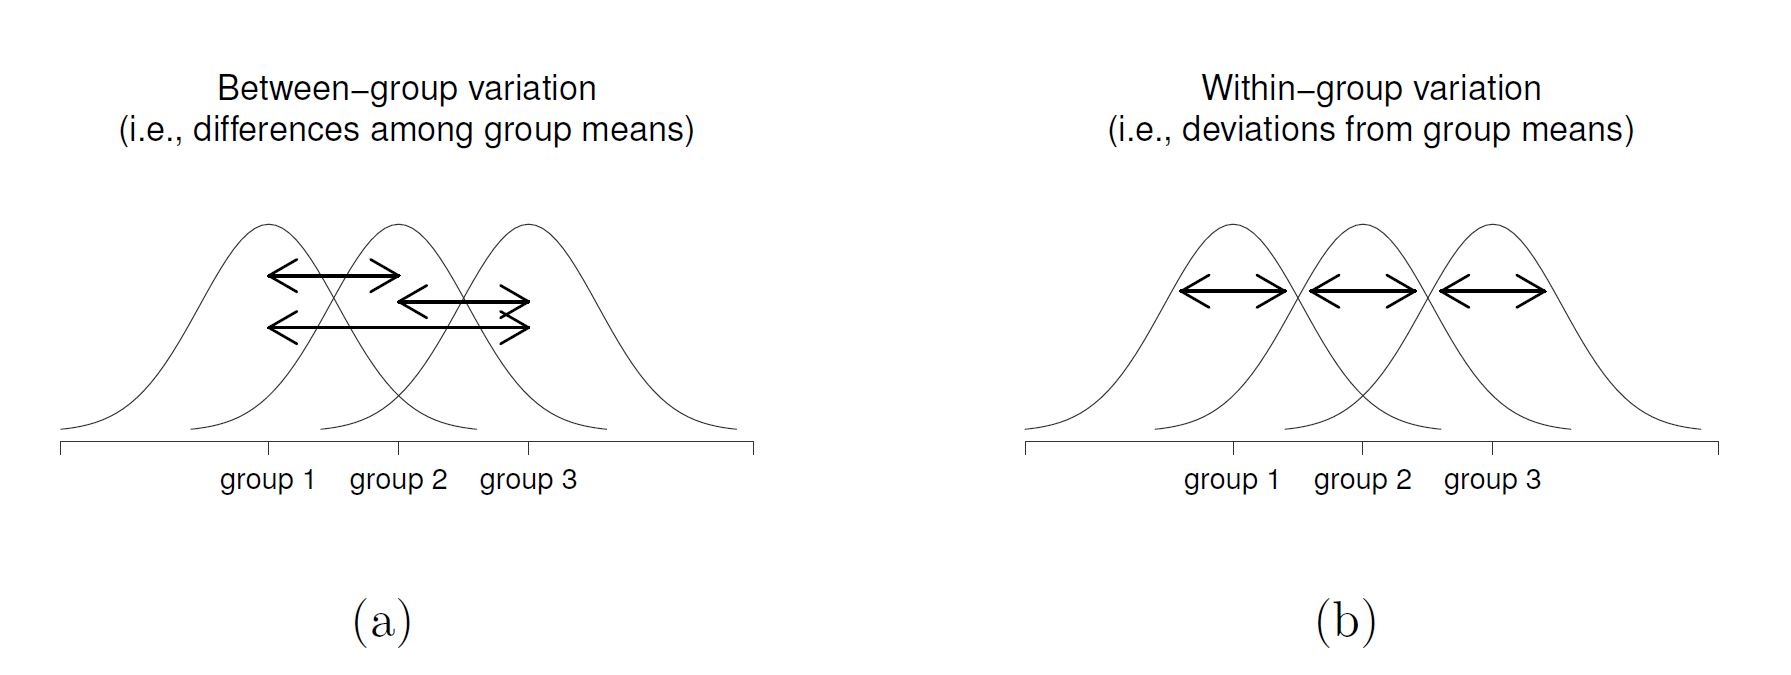
\includegraphics[width=0.8\linewidth]{images/04_one-way-anova/anova graphic} 

}

\caption{Graphical illustration of the one-way ANOVA}\label{fig:unnamed-chunk-1}
\end{figure}

\hypertarget{an-example-with-the-math}{%
\subsection{An example with the math}\label{an-example-with-the-math}}

In case it's useful, read below. If your eyes are glazing over, just move to the next section.

You can read the example dataset below. I've pulled the relevant data here so we can go through a hand calculation ourselves.

\begin{longtable}[]{@{}llll@{}}
\toprule
\begin{minipage}[b]{0.17\columnwidth}\raggedright
Drug\strut
\end{minipage} & \begin{minipage}[b]{0.11\columnwidth}\raggedright
N\strut
\end{minipage} & \begin{minipage}[b]{0.16\columnwidth}\raggedright
Mean\strut
\end{minipage} & \begin{minipage}[b]{0.16\columnwidth}\raggedright
Variance\strut
\end{minipage}\tabularnewline
\midrule
\endhead
\begin{minipage}[t]{0.17\columnwidth}\raggedright
Anxifree\strut
\end{minipage} & \begin{minipage}[t]{0.11\columnwidth}\raggedright
6\strut
\end{minipage} & \begin{minipage}[t]{0.16\columnwidth}\raggedright
0.7167\strut
\end{minipage} & \begin{minipage}[t]{0.16\columnwidth}\raggedright
.1537\strut
\end{minipage}\tabularnewline
\begin{minipage}[t]{0.17\columnwidth}\raggedright
Joyzepam\strut
\end{minipage} & \begin{minipage}[t]{0.11\columnwidth}\raggedright
6\strut
\end{minipage} & \begin{minipage}[t]{0.16\columnwidth}\raggedright
1.4833\strut
\end{minipage} & \begin{minipage}[t]{0.16\columnwidth}\raggedright
.0457\strut
\end{minipage}\tabularnewline
\begin{minipage}[t]{0.17\columnwidth}\raggedright
Placebo\strut
\end{minipage} & \begin{minipage}[t]{0.11\columnwidth}\raggedright
6\strut
\end{minipage} & \begin{minipage}[t]{0.16\columnwidth}\raggedright
0.4500\strut
\end{minipage} & \begin{minipage}[t]{0.16\columnwidth}\raggedright
.0790\strut
\end{minipage}\tabularnewline
\begin{minipage}[t]{0.17\columnwidth}\raggedright
\textbf{Overall}\strut
\end{minipage} & \begin{minipage}[t]{0.11\columnwidth}\raggedright
\textbf{18}\strut
\end{minipage} & \begin{minipage}[t]{0.16\columnwidth}\raggedright
\textbf{0.8833}\strut
\end{minipage} & \begin{minipage}[t]{0.16\columnwidth}\raggedright
\textbf{.28}\strut
\end{minipage}\tabularnewline
\bottomrule
\end{longtable}

Let's start with the easy stuff! Let's calculate our degrees of freedom.

\(df_{BG} = k - 1 = 3 -1 = 2\)

\(df_{WG} = N - k = 18 - 3 = 15\)

Now let's move to the more complicated ones.

\(\begin{aligned} SS_{BG} &= \sum{n_k}(\bar{X_k}-\bar{X}_{grand})^2 \\ SS_{BG} &= 6(.7167-.8833)^2 + 6(1.4833-.8833)^2 + 6(.4500-.8833)^2 \\ SS_{BG} &= 6(-.1666)^2 + 6(.6)^2 + 6(-.4333)^2 \\ SS_{BG} &= 6(.0278) + 6(.36) + 6(.1877) \\ SS_{BG} &= .1665 + 2.16 + 1.1262 \\ SS_{BG} &= 3.453 \end{aligned}\)

Then we can calculate our \(MS_{BG}\).

\(MS_{BG} = \frac{SS_{BG}}{df_{BG}} = \frac{3.453}{2} = 1.727\)

Let's move to our \(SS_{WG}\).

\(\begin{aligned} SS_{WG} &= \sum{s_k^2}(n_k - 1) \\ SS_{WG} &= .1537(6-1) + .0457(6-1) + .0790(6-1) \\ SS_{WG} &= .1537(5) + .0457(5) + .0790(5) \\ SS_{WG} &= .7685 + .2285 + .3950 \\ SS_{WG} &= 1.392 \end{aligned}\)

Now we can calculate our \(MS_{WG}\).

\(MS_{WG} = \frac{SS_{WG}}{df_{WG}} = \frac{1.392}{15} = .0928\)

Now all that's left is to calculate \(F\)!

\(F = \frac{MS_{BG}}{MS_{WG}} = \frac{1.726}{.0928} = 18.60\)

Compare to the \(F\), \(df_{WG}\), and \(df_{BG}\) in the output below in jamovi! Notice how close we are. Also notice how many decimals I retained throughout the analyses. I was a bit off when I first did this with only two decimals throughout. Retaining four decimals throughout got me only \textasciitilde one-hundredth of a decimal off from the actual results. Neat!

\hypertarget{assumptions-2}{%
\section{Assumptions}\label{assumptions-2}}

As a parametric test, the one-way ANOVA has the same assumptions as other parametric tests:

\begin{enumerate}
\def\labelenumi{\arabic{enumi}.}
\item
  The dependent variable is \textbf{normally distributed}
\item
  Variances in the two groups are roughly equal (i.e., \textbf{homogeneity of variances})
\item
  The dependent variable is \textbf{interval or ratio} (i.e., continuous)
\item
  Scores are \textbf{independent} between groups
\end{enumerate}

We cannot \underline{test} the third and fourth assumptions; rather, those are based on knowing your data. However, we can and should test for the first two assumptions. Fortunately, the one-way ANOVA in jamovi has three check boxes under ``Assumption Checks'' that lets us test for both assumptions.

\hypertarget{anova-is-robust-to-violations}{%
\subsection{ANOVA is robust to violations}\label{anova-is-robust-to-violations}}

Although we should meet the assumptions as much as possible, in general the F-statistic is \emph{robust} to violations of normality and homogeneity of variance. This means that you can still run the one-way ANOVA if you violate the assumptions, but \emph{only when group sizes are equal or nearly equal}. If you have vastly different variances (such as 2:1 ratio or greater) or vastly different group sizes (such as a 2:1 ratio or greater), and especially if one group is small (such as 10 or fewer cases), then your F-statistic is likely to be very wrong. For example, if your larger group has the larger variance, then your F-statistic is likely to be non-significant or smaller than it should be; however, if your larger group has smaller variance,then your F-statistic is likely to be significant or bigger than it should be!

\hypertarget{in-jamovi-2}{%
\section{In jamovi}\label{in-jamovi-2}}

Let's run an example with data from lsj-data. Open data from your Data Library in ``lsj-data''. Select and open ``clinicaltrial''. This dataset is hypothetical data of a clinical trial in which you are testing a new antidepressant drug called \emph{Joyzepam}. In order to construct a fair test of the drug's effectiveness, the study involves three separate drugs to be administered. One is a placebo, and the other is an existing antidepressant / anti-anxiety drug called \emph{Anxifree}. A collection of 18 participants with moderate to severe depression are recruited for your initial testing. Because the drugs are sometimes administered in conjunction with psychological therapy, your study includes 9 people undergoing cognitive behavioral therapy (CBT) and 9 who are not. Participants are randomly assigned (doubly blinded, of course) a treatment, such that there are 3 CBT people and 3 no-therapy people assigned to each of the 3 drugs. A psychologist assesses the mood of each person after a 3 month run with each drug, and the overall improvement in each person's mood is assessed on a scale ranging from -5 to +5.

\begin{enumerate}
\def\labelenumi{\arabic{enumi}.}
\item
  To perform a one-way ANOVA in jamovi, go to the Analyses tab, click the ANOVA button, and choose ``ANOVA''. You might be asking why we aren't choosing ``One-Way ANOVA'' and that's because the options there are too limited.
\item
  Move your dependent variable \texttt{mood.gain} to the Dependent Variable box and your independent variable \texttt{drug} to the Fixed Factors box.
\item
  Select \(\omega^2\) for your effect size.
\item
  Ignore the Model drop-down menu. If you are doing more complicated ANOVAs you will need this. We will ignore it.
\item
  In the Assumption Checks drop-down menu, select all three options: \texttt{Homogeneity\ test}, \texttt{Normality\ test}, and \texttt{Q-Q\ plot}.
\item
  Ignore the Contrasts and Post Hoc Tests drop-down menus for now. See below for more information on them.
\item
  Ignore the Estimated Marginal Means drop-down menu.
\end{enumerate}

When you are done, your setup should look like this:

\begin{figure}

{\centering 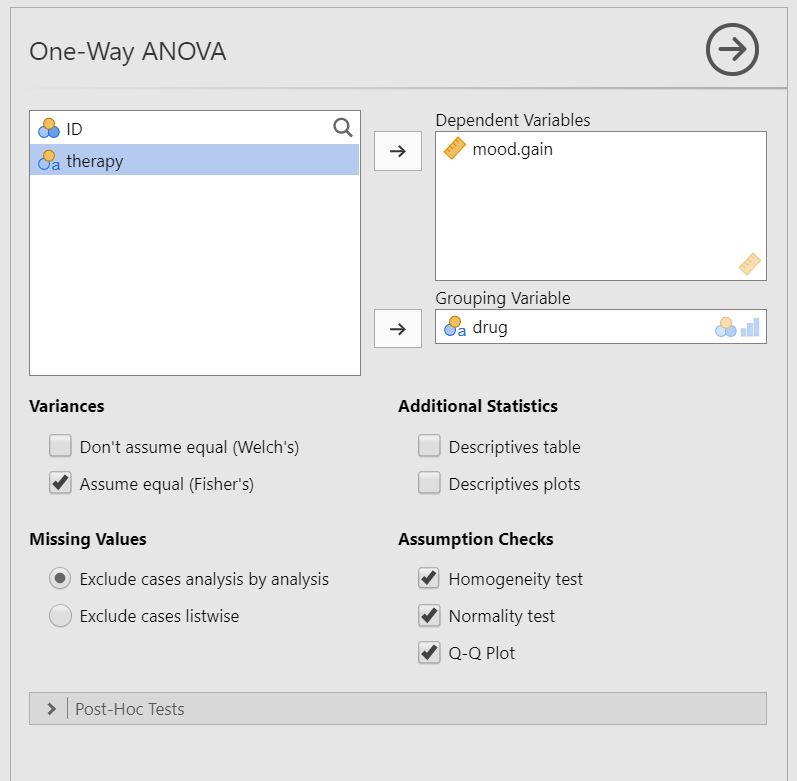
\includegraphics[width=0.8\linewidth]{images/04_one-way-anova/one-way_setup} 

}

\caption{One-way ANOVA setup in jamovi}\label{fig:unnamed-chunk-2}
\end{figure}

\hypertarget{checking-assumptions-in-jamovi-2}{%
\subsection{Checking assumptions in jamovi}\label{checking-assumptions-in-jamovi-2}}

We test for normality using the Shapiro-Wilk test and the Q-Q plot. The Shapiro-Wilk test was not statistically significant (W = .96, \emph{p} = .605); therefore, this indicates the data is normally distributed. Furthermore, the lines are fairly close to the diagonal line in the Q-Q plot. We can conclude that we satisfy the assumption of normality.

We test for homogeneity of variance using the Levene's test. The Levene's test was not statistically significant (\emph{F} {[}2, 15{]} = 1.45, \emph{p} = .266); therefore, this indicates our data satisfies the assumption of homogeneity of variance. However, I would add a caveat that we have a small sample of data (\emph{N} = 18); we should have tried to collect more data.

\begin{figure}

{\centering 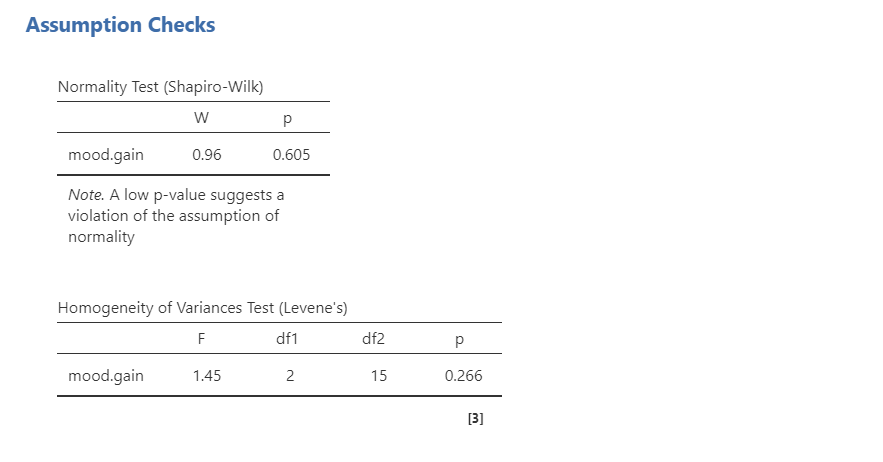
\includegraphics[width=1\linewidth]{images/04_one-way-anova/one-way_assumptions1} 

}

\caption{Testing assumptions in jamovi}\label{fig:unnamed-chunk-3}
\end{figure}

\begin{figure}

{\centering 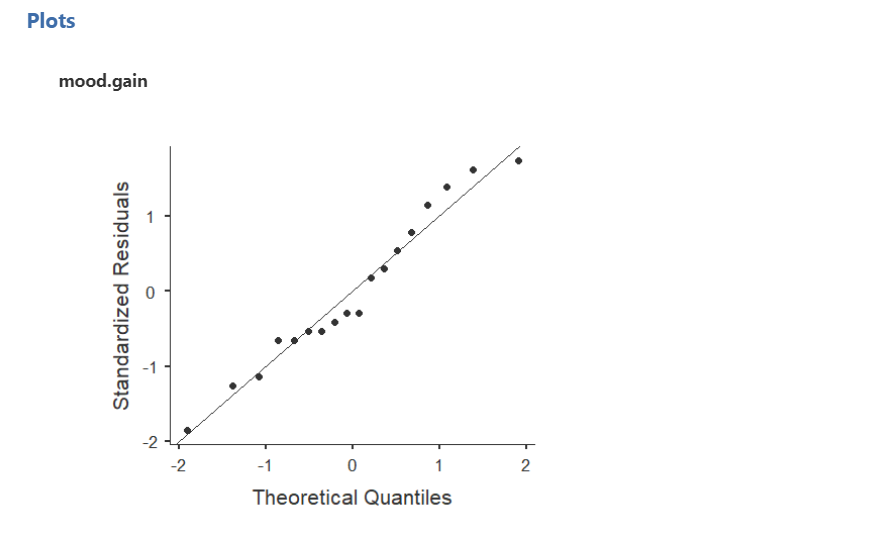
\includegraphics[width=1\linewidth]{images/04_one-way-anova/one-way_assumptions2} 

}

\caption{**CAPTION THIS FIGURE!!**}\label{fig:unnamed-chunk-4}
\end{figure}

\hypertarget{interpreting-results-2}{%
\section{Interpreting results}\label{interpreting-results-2}}

Once we are satisfied we have satisfied the assumptions for the independent t-test, we can interpret our results.

\begin{figure}

{\centering 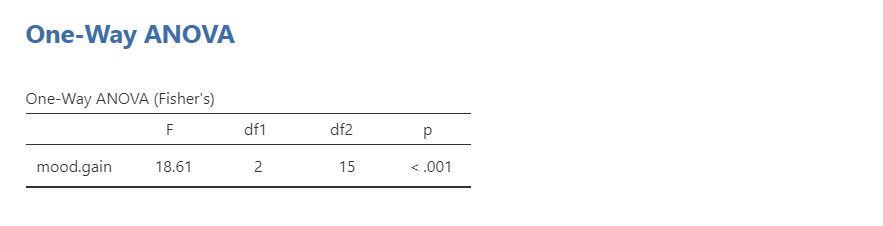
\includegraphics[width=1\linewidth]{images/04_one-way-anova/one-way_results} 

}

\caption{One-way ANOVA results in jamovi}\label{fig:unnamed-chunk-5}
\end{figure}

Our p-value is less than .05, so our results are statistically significant. We can write up our results in APA something like this:

\begin{quote}
There is a significant difference in mood gain across the three drug conditions, \emph{F} (2, 15) = 18.61, \emph{p} \textless{} .001, \(\omega^2\) = .66.
\end{quote}

Sometimes, people like to put the statistics inside a parentheses. In that case, you need to change the parentheses around the degrees of freedom as brackets. Here's another example write-up of the results in APA style:

\begin{quote}
There is a significant difference in mood gain across the three drug conditions (\emph{F} {[}2, 15{]} = 18.61, \emph{p} \textless{} .001, \(\omega^2\) = .66).
\end{quote}

\hypertarget{a-note-on-one-tailed-vs.-two-tailed-tests}{%
\subsection{A note on one-tailed vs.~two-tailed tests}\label{a-note-on-one-tailed-vs.-two-tailed-tests}}

Unlike a t-test, we would not halve the p-value in an F-ratio because it is an omnibus test. Our planned contrasts or post-hoc tests can tell us where differences are, and we can provide directional hypotheses there if we so choose.

\hypertarget{what-if-i-violated-assumptions-2}{%
\section{What if I violated assumptions?}\label{what-if-i-violated-assumptions-2}}

The great news is that jamovi includes the Welch's F-statistic and the Kruskal-Wallis non-parametric test! The bad news is that you lose some functionality in jamovi when you use them. Just like with the Welch's t-statistic (for the independent t-test), it does not have the assumption of equal variances so it's appropriate to use if your data is normally distributed but does not have homogeneous variances. Similarly, the Kruskal-Wallis test is the non-parametric version of the one-way ANOVA and should be used if you do not satisfy the assumption of normality.

Here's what statistic you should choose based on satisfying assumptions:

\begin{longtable}[]{@{}lll@{}}
\toprule
\begin{minipage}[b]{0.40\columnwidth}\raggedright
\strut
\end{minipage} & \begin{minipage}[b]{0.24\columnwidth}\raggedright
\textbf{Normality: satisfied}\strut
\end{minipage} & \begin{minipage}[b]{0.27\columnwidth}\raggedright
\textbf{Normality: not satisfied}\strut
\end{minipage}\tabularnewline
\midrule
\endhead
\begin{minipage}[t]{0.40\columnwidth}\raggedright
\textbf{Homogeneity of Variance: satisfied}\strut
\end{minipage} & \begin{minipage}[t]{0.24\columnwidth}\raggedright
one-way ANOVA\strut
\end{minipage} & \begin{minipage}[t]{0.27\columnwidth}\raggedright
Kruskal-Wallis\strut
\end{minipage}\tabularnewline
\begin{minipage}[t]{0.40\columnwidth}\raggedright
\textbf{Homogeneity of Variance: not satisfied}\strut
\end{minipage} & \begin{minipage}[t]{0.24\columnwidth}\raggedright
Welch's F-test\strut
\end{minipage} & \begin{minipage}[t]{0.27\columnwidth}\raggedright
Kruskal-Wallis\strut
\end{minipage}\tabularnewline
\bottomrule
\end{longtable}

\hypertarget{welchs-f-test-in-jamovi}{%
\subsubsection{Welch's F-test in jamovi}\label{welchs-f-test-in-jamovi}}

To conduct this in jamovi, you will need to use the ``One-Way ANOVA'' test, not the ``ANOVA'' test. The unfortunate thing about this test is that it strangely does not provide effect sizes.

In jamovi, under Variances select \texttt{Don\textquotesingle{}t\ assume\ equal\ (Welch\textquotesingle{}s)}. Move \texttt{mood.gain} to the Dependent Variable box and \texttt{drug} to your Grouping Variable box. You will interpret the results similarly to the one-way ANOVA:

\begin{figure}

{\centering 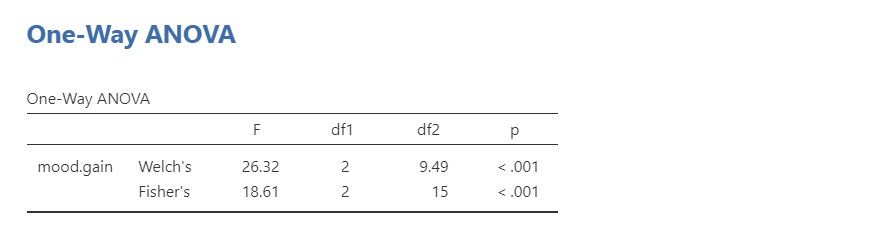
\includegraphics[width=1\linewidth]{images/04_one-way-anova/one-way_results_Welch} 

}

\caption{One-way ANOVA results in jamovi}\label{fig:unnamed-chunk-6}
\end{figure}

\begin{quote}
Using a Welch's F-test, there is a significant difference in mood gain across the three drug conditions, \emph{F} (2, 9.49) = 26.32, \emph{p} \textless{} .001.
\end{quote}

\hypertarget{kruskal-wallis-test-in-jamovi}{%
\subsubsection{Kruskal-Wallis test in jamovi}\label{kruskal-wallis-test-in-jamovi}}

To perform the Kruskal-Wallis test in jamovi, you will need to select under the ANOVA button ``One-Way ANOVA, Kruskal Wallis'' towards the bottom of the list of options. Move \texttt{mood.gain} to the Dependent Variables box and \texttt{drug} to the Grouping Variable box. Select Effect size; if you need post hoc comparisons select DSCF pairwise comparisons (see section below on group differences). You will interpret the results similarly to the one-way ANOVA:

\begin{figure}

{\centering 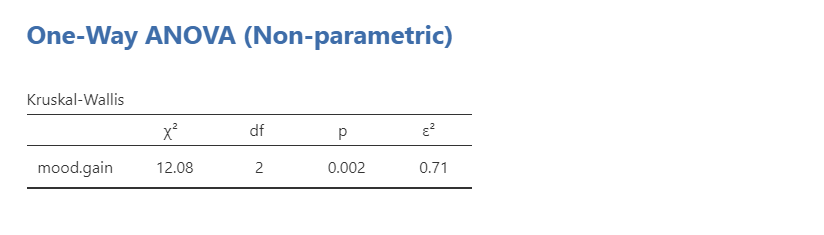
\includegraphics[width=1\linewidth]{images/04_one-way-anova/one-way_results_Kruskal} 

}

\caption{Kruskal-Wallis results in jamovi}\label{fig:unnamed-chunk-7}
\end{figure}

\begin{quote}
Using a Kruskal-Wallis test, there is a significant difference in mood gain across the three drug conditions, \(\chi^2\) (2) = 12.08, \emph{p} = .002, \(\epsilon^2\) = .71.
\end{quote}

Notice how in this case all three results converge and show there is a statistically significant difference in the results! The problem is\ldots{} differences in which groups?

\hypertarget{finding-group-differences}{%
\section{Finding Group Differences}\label{finding-group-differences}}

Often, we're not interested in just \emph{whether} there is a difference (which the F-statistic can tell us), but \emph{where} the differences are between groups (which the F-statistic cannot tell us). For that, we use either \underline{planned contrasts} when you have specific hypotheses you want to test or \underline{post-hoc comparisons} when you have no specific hypotheses.

\textbf{Note}: You \underline{do not} perform contrasts or post hoc comparisons if your overall \(F\) statistic is not statistically significant. You do not interpret group differences if you fail to reject the null hypothesis that there are no group differences!

\hypertarget{planned-contrasts}{%
\subsection{Planned Contrasts}\label{planned-contrasts}}

If you have before-analysis hypotheses of group differences in your data, you will use planned contrasts. You can find the planned contrasts in the ANOVA (but not the one-way ANOVA) setup as a drop-down menu. Note that while I show all six contrasts that jamovi provides, you do not normally do multiple contrasts. These are just shown for illustrative purposes:

\begin{enumerate}
\def\labelenumi{\arabic{enumi}.}
\tightlist
\item
  \textbf{Deviation}: compares the effect of each category (except the first category) to the overall experimental effect. The order of categories is alphabetical or numerical order. Notice how anxifree is considered the first category.
\end{enumerate}

\begin{figure}

{\centering 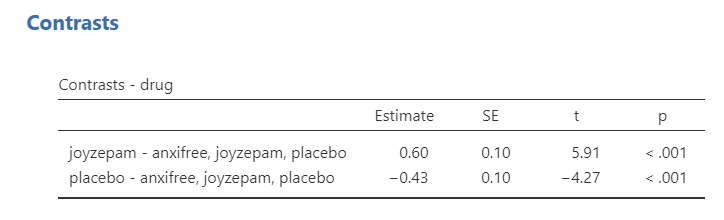
\includegraphics[width=1\linewidth]{images/04_one-way-anova/contrasts_deviation} 

}

\caption{**CAPTION THIS FIGURE!!**}\label{fig:unnamed-chunk-8}
\end{figure}

\begin{enumerate}
\def\labelenumi{\arabic{enumi}.}
\setcounter{enumi}{1}
\tightlist
\item
  \textbf{Simple}: Each category is compared to the first category. The order of categories is alphabetical or numerical order. Notice how anxifree is considered the first category.
\end{enumerate}

\begin{figure}

{\centering 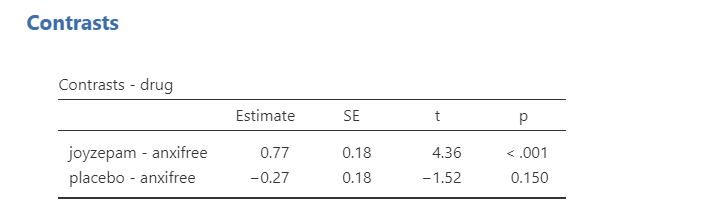
\includegraphics[width=1\linewidth]{images/04_one-way-anova/contrasts_simple} 

}

\caption{**CAPTION THIS FIGURE!!**}\label{fig:unnamed-chunk-9}
\end{figure}

\begin{enumerate}
\def\labelenumi{\arabic{enumi}.}
\setcounter{enumi}{2}
\tightlist
\item
  \textbf{Difference}: Each category (except the first) is compared to the mean effect of all previous categories.
\end{enumerate}

\begin{figure}

{\centering 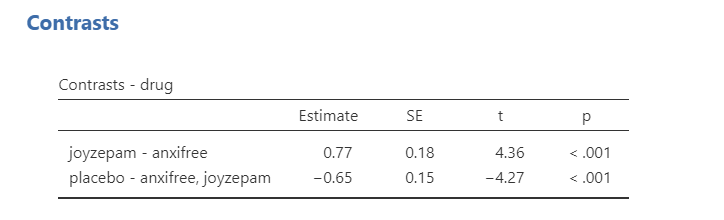
\includegraphics[width=1\linewidth]{images/04_one-way-anova/contrasts_difference} 

}

\caption{**CAPTION THIS FIGURE!!**}\label{fig:unnamed-chunk-10}
\end{figure}

\begin{enumerate}
\def\labelenumi{\arabic{enumi}.}
\setcounter{enumi}{3}
\tightlist
\item
  \textbf{Helmert}: Each category (except the last) is compared to the mean effect of all subsequent categories.
\end{enumerate}

\begin{figure}

{\centering 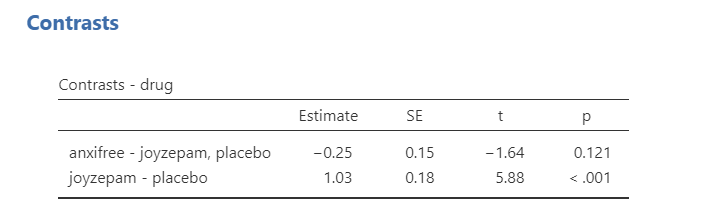
\includegraphics[width=1\linewidth]{images/04_one-way-anova/contrasts_helmert} 

}

\caption{**CAPTION THIS FIGURE!!**}\label{fig:unnamed-chunk-11}
\end{figure}

\begin{enumerate}
\def\labelenumi{\arabic{enumi}.}
\setcounter{enumi}{4}
\tightlist
\item
  \textbf{Repeated}: Each category is compared to the last category.
\end{enumerate}

\begin{figure}

{\centering 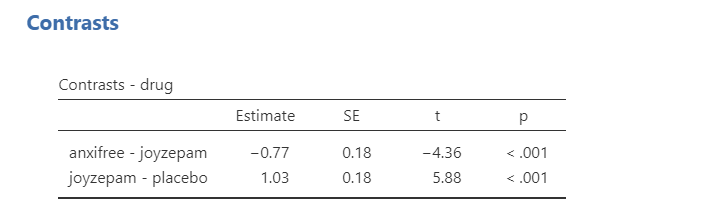
\includegraphics[width=1\linewidth]{images/04_one-way-anova/contrasts_repeated} 

}

\caption{**CAPTION THIS FIGURE!!**}\label{fig:unnamed-chunk-12}
\end{figure}

\begin{enumerate}
\def\labelenumi{\arabic{enumi}.}
\setcounter{enumi}{5}
\tightlist
\item
  \textbf{Polynomial}: Tests trends in the data. It will examine the \emph{n-1}\textsuperscript{th} degree based on the number of groups. In this case, because we have 3 groups it is testing both a linear (\textsuperscript{1}) and quadratic (\textsuperscript{2}) trend. If we had 5 groups, it would test a linear (\textsuperscript{1}), quadratic (\textsuperscript{2}), cubic (\textsuperscript{3}), and quartic (\textsuperscript{4}) trend. Note that your factor levels must be ordinal for a polynomial contrast to make sense.
\end{enumerate}

\begin{figure}

{\centering 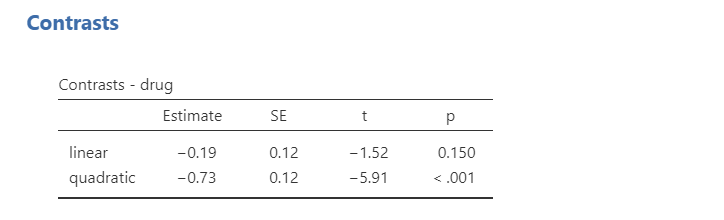
\includegraphics[width=1\linewidth]{images/04_one-way-anova/contrasts_polynomial} 

}

\caption{**CAPTION THIS FIGURE!!**}\label{fig:unnamed-chunk-13}
\end{figure}

\textbf{Test yourself!} Which contrast would make \underline{most sense} to test given that we want to know how our drug compares to the other two drugs? deviation simple difference helmert repeated polynomial

\hypertarget{writing-up-planned-contrasts}{%
\subsubsection{Writing up planned contrasts}\label{writing-up-planned-contrasts}}

Here's some example write-ups of the above results.

\begin{quote}
There is a significant difference in mood gain across the three drug conditions, \emph{F} (2, 15) = 18.61, \emph{p} \textless{} .001. Repeated contrasts showed that \emph{Joyzepam} (\emph{M} = 1.48, \emph{SD} = .21) outperformed both \emph{Anxifree} (\emph{M} = .72, \emph{SD} = .39; \emph{p} \textless{} .001) and the placebo condition (\emph{M} = .45, \emph{SD} = .28; \emph{p} \textless{} .001).

(Note how this example makes no sense because our data is not ordinal) There is a significant difference in mood gain across the three drug conditions, \emph{F} (2, 15) = 18.61, \emph{p} \textless{} .001. There was not a significant linear trend across the drug conditions (\emph{p} = .150).
\end{quote}

\hypertarget{post-hoc-comparisons}{%
\subsection{Post hoc comparisons}\label{post-hoc-comparisons}}

Often, we do not have any \emph{a priori} (or planned) predictions or hypotheses about our group differences. In this case, we use post hoc procedures. These procedures do \underline{pairwise comparisons} among all of our groups, like t-tests across each of our groups. As we noted on the first page of this handout, this can be highly problematic for our Type I error rate! Therefore, we must perform corrections to control our familywise error rate.

jamovi currently supports five types of post-hoc tests; I generally only use Tukey or Bonferonni:

\begin{enumerate}
\def\labelenumi{\arabic{enumi}.}
\tightlist
\item
  \textbf{No correction}: This doesn't correct for a Type I error at all. Don't use this! I won't even show it. It's bad. Never use it. NEVER. You are warned!
\item
  \textbf{Tukey}: This is the post hoc test I use most often. It controls the Type I error rate well, but isn't as conservative of a control as the Bonferonni.
\item
  \textbf{Scheffe}: Honestly, I've never used it. I am not sure how it's calculated.
\item
  \textbf{Bonferroni}: This is the most conservative test. It's good if you only have a small number of comparisons to make or if you \emph{really} want to control your Type I error rate. If you have a lot of them to test , then you should use something else.
\item
  \textbf{Holm}: Honestly, I've never used it. I am not sure how it's calculated.
\end{enumerate}

Games-Howell for when you have unequal variances and Tukey for when you have equal variances. They will each calculate your p-values slightly differently but in a way to control for our Type I error rate as best it can. They are interpreted very similarly, so we will proceed with the Tukey's post hoc comparisons because we satisfied the assumption of equal variances.

To request post hoc tests from the one-way ANOVA, open the collapsed menu at the bottom of the setup menu. Select \texttt{Tukey\ (equal\ variances} under Post-Hoc Test and select \texttt{Mean\ difference}, \texttt{Report\ significance}, and \texttt{Flag\ significant\ comparisons} under Statistics. Optionally, you can request the \texttt{Test\ results\ (t\ and\ df)} although this is not necessary.

Below shows the post hoc test results for our one-way ANOVA. Notice the differences in p-values across the four post hoc tests and how all other values are the same. Notice how the Bonferroni is most conservative (i.e., has the largest p-values) and the Holm's is the least conservative (i.e., has the smallest p-values). Keep in mind you do not normally ask for multiple post hoc comparisons. Just pick one! Normally, I just pick Tukey's.

\begin{figure}

{\centering 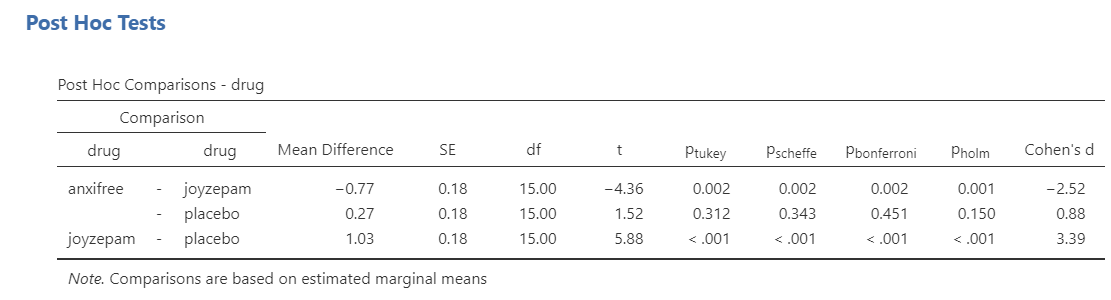
\includegraphics[width=1\linewidth]{images/04_one-way-anova/one-way_results_post-hoc} 

}

\caption{Post hoc test results in jamovi}\label{fig:unnamed-chunk-14}
\end{figure}

\hypertarget{writing-up-post-hoc-results}{%
\subsubsection{Writing up post hoc results}\label{writing-up-post-hoc-results}}

The way we would write up each of the post hoc comparisons is very similar. Given that I usually use Tukey, here is a write-up for those results:

\begin{quote}
There is a significant difference in mood gain across the three drug conditions, \emph{F} (2, 15) = 18.61, \emph{p} \textless{} .001. Post hoc comparisons using Tukey's HSD revealed that our drug \emph{Joyzepam} (\emph{M} = 1.48, \emph{SD} = .21) outperformed both \emph{Anxifree} (\emph{M} = .72, \emph{SD} = .39; \emph{p} = .002) and the placebo condition (\emph{M} = .45, \emph{SD} = .28; \emph{p} \textless{} .001); there were no differences between \emph{Anxifree} and the placebo condition (\emph{p}
\end{quote}

\hypertarget{group-differences-with-violated-assumptions}{%
\subsection{Group differences with violated assumptions}\label{group-differences-with-violated-assumptions}}

If you are using Welch's F-test using the One-Way ANOVA in jamovi, you should select under Post-Hoc Tests \texttt{Games-Howell\ (unequal\ variances)}. These will be interpreted similarly to the post hoc comparisons above.

If you are using the Kruskal-Wallis test, you will select the check-box for \texttt{DSCF\ pairwise\ comparisons}. This stands for the Dwass-Steel-Critchlow-Fligner test. All you need to know is that they, too, are interpreted similarly to the post hoc comparisons above.

Unfortunately, you cannot perform contrasts with either the Welch's F-test or Kruskal-Wallis test.

\hypertarget{tips-on-writing-up-results}{%
\section{Tips on writing up results}\label{tips-on-writing-up-results}}

Writing up results in APA style is both a science and an art. There's a science to what you need to report. For example, you always report the statistics exactly the same: \emph{F} (df\textsubscript{WG}, df\textsubscript{BG}) = X.XX, \emph{p} = .XXX. You also always report the group means (\emph{M}) and standard deviations (\emph{SD}), although you can report them in-text like I did above or in a descriptives table like you can ask from jamovi.

However, there's also an art to it. Notice how I wrote that up in a way to summarize the findings as succinctly as possible. I could have said there was a difference between \emph{anxifree} and \emph{joyzepam} and a difference between \emph{joyzepam} and the placebo, but that's a lot more words and isn't written in a way to focus on what I'm hoping to see: that my drug \emph{joyzepam} performed better than the competitor \emph{anxifree} and a placebo condition.

This is where you need to think creatively and be very critical in checking that what you say makes sense. Read your write-ups carefully! Have someone else read it. Can they understand what you mean?

\hypertarget{your-turn-2}{%
\section{Your turn!}\label{your-turn-2}}

Open the \texttt{Sample\_Dataset\_2014.xlsx} file that we will be using for all Your Turn exercises.

Perform one-way ANOVAs based on the following research questions. Check your assumptions and ensure you are using the correct tests.

To get the most out of these exercises, try to first find out the answer on your own and then use the drop-down menus to check your answer.

\begin{enumerate}
\def\labelenumi{\arabic{enumi}.}
\item
  \textbf{Does students differ on English scores by rank (i.e., freshmen, sophomore, junior, senior)?}

  \begin{itemize}
  \item
    Do you satisfy the assumption of normality? yes no
  \item
    Do you satisfy the assumption of homogeneity of variance? yes no
  \item
    Which statistic should you use? one-way ANOVA Welch's F-test Kruskal-Wallis test
  \item
    Do students differ on English scores by rank? yes no
  \item
    Should you perform a planned contrast or post hoc comparison? yes no
  \item
    What are the results of the post hoc comparison? N/A - Don't perform Freshmen had higher English scores than sophomores, juniors, and seniors Freshmen and sophomores had higher English scores than juniors and seniors
  \end{itemize}
\item
  \textbf{Does smoking status (Smoking: Nonsmoker = 0, Past smoker = 1, Current smoker = 2) relate to sprint time?}

  \begin{itemize}
  \item
    Do you satisfy the assumption of normality? yes no
  \item
    Do you satisfy the assumption of homogeneity of variance? yes no
  \item
    Which statistic should you use? one-way ANOVA Welch's F-test Kruskal-Wallis test
  \item
    Does smoking status relate to sprint time? yes no
  \item
    Should you perform a planned contrast or post hoc comparison? yes no
  \item
    What are the results of the post hoc comparison? N/A - Don't perform Nonsmokers had significantly faster sprint times than current smokers Nonsmokers and past smokers had significantly faster spring times than current smokers Nonsmokers had significantly faster sprint times than both past and current smokers
  \end{itemize}
\end{enumerate}

\hypertarget{appendix-appendices}{%
\appendix}


\hypertarget{references}{%
\chapter{References}\label{references}}

  \bibliography{book.bib,packages.bib}

\end{document}
